\subsection{Website fingerprinting}
We have to overcome the following problems:
\begin{itemize}
	\item DNS sniffing only tells us what \emph{domains}, but not what
		\emph{pages} a user visits.  Can be a big problem, e.g., with Wikipedia.
	\item DNS records are cached by the resolver for the duration of the TTL.
\end{itemize}

The following aspects might work in our favor:
\begin{itemize}
	\item When visiting a page, your browser sends \emph{multiple} DNS queries.
	\item In tor, the DNS cache enforces a minimum TTL of 60 seconds and a maximum
	TTL of 30 minutes (see tor/src/or/dns.c:278).
	\item If we can observe the DNS requests from the exit the user is
	using (this is the case only with some probability, \eg 22\% for
	the Google adversary?) and account for caching (by including all
	requests from the last 30 minutes), the ``size of the world'' is
	reduced drastically. In other words, the attack game changes from an
	open-world to a closed-world setting. (This holds probably only for
	web\emph{site} fingerprinting, not web\emph{page} fingerprinting.)
\end{itemize}

We gathered five samples of Alexa top 10,000 sites using Firefox 38.7.1 ESR
configured like TBB 5.5.4 and recorded all DNS requests and responses.
We found 59,842 unique domains that only appear on one site, with the per site
number of unique domains mean 6, std 5.6, median 4, min 0, and max 118.
98.2\% out of all sites have unique domains.
Figure~\ref{fig:dns-unique-domains-ff} shows the distribution of sites
without unique domains. Primarily sites in the top 100 of Alexa lacks unique
domains. Applying the Tor cache enforced minimum and maxium TTL, the unique
domain minimum TTL for each site with unique domains have mean 353.6, std 522.0,
median 60, min 60, and max 1800. In other words: for half of the sites in
Alexa top-10,000, there is at least one unique domain with TTL 60 seconds.
This means that if the site has not been requested within the last minute
by a tor exit then the tor exit will send at least one DNS request containing
a uniquely identifying domain for half of the sites in Alexa top-10,000.

\begin{figure}[t]
	\centering
	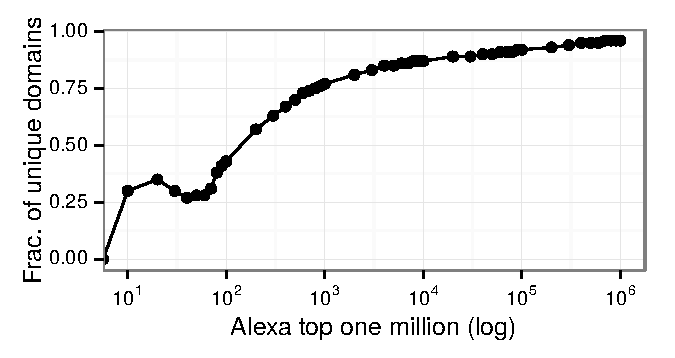
\includegraphics[width=\linewidth]{figures/dns-unique-domains}
	\caption{The distribution of site on Alexa top 10,000 without unique domains.
	Gathered March 25-27 2016 with five samples.}
	\label{fig:dns-unique-domains-ff}
\end{figure}

Other facts that are relevant here:
\begin{itemize}
	\item Tor Browser does not prefetch domain names, but content providers can
	make Tor Browser resolve arbitrary domains by including images or scripts
	with sources of their choice into pages. 
\end{itemize}
